\subsection{Multi-Factor Models}

\begin{definition} \hlt{Arbitrage Pricing Theory (APT)}\\
Alternative to CAPM. Linear model with multiple systematic risk factors priced by market.\\
APT does not identify specific risk factors or number of factors.
\begin{equation}
E[r_p] = r_f + \sum\limits_{j=1}^{K} \beta_{p,j} r_{j} + \epsilon_i \nonumber
\end{equation}
where $r_i$ is return on portfolio $p$, $r_f$ is risk-free rate, $r_j$ is expected risk premium of risk factor $\beta_{p,j}$.
\end{definition}

\begin{remark} \hlt{Arbitrage Pricing Theory Assumptions (APT)}
\begin{enumerate}[label=\roman*.]
\setlength{\itemsep}{0pt}
\item Asset-specific risk may be diversified away in a portfolio.
\item Returns are generated with a factor model.
\item No arbitrage opportunities exist among well-diversified portfolio.
\end{enumerate}
\end{remark}

\begin{remark} \hlt{Arbitrage in APT}\\
Long assets with high ratio of return-per-unit-of-factor-exposure, short assets with low return-per-unit-of-factor-exposure. i.e., long portfolio with same beta but higher expected return, short that with lower expected return.\\
Such arbitrage opportunities will be exploited and eliminated immediately.
\end{remark}

\begin{remark} \hlt{Types of Multi-Factor Models}
\begin{enumerate}[label=\roman*.]
\setlength{\itemsep}{0pt}
\item Macroeconomic Factor Models: returns are explained by surprises in macroeconomic risk factors (i.e., GDP, interest rates, inflation). Factor surprises is the difference between realised value of the factor and its consensus predicted value. Note that the variables that explain the return is not the value of the variables itself, but the unexpected component, as the expected value has already been reflected in prices.
\item Fundamental Factor Models: returns are explained by multiple firm-specific factors (i.e., P/E ratio, market cap, leverage ratio, earnings growth rate)
\item Statistical Factor Models: statistical methods used to explain asset returns. In factor analysis, factors are portfolios that explain covariance in asset returns. In principal component models, factors are portfolios that explain the variance in asset returns. Statistical factors do not lend well to economic interpretation. 
\end{enumerate}
\end{remark}

\begin{definition} \hlt{Macroeconomic Factor Models}\\
An example of two-factor macroeconomic model in which stock prices are explained by surprises in GDP growth rates and credit quality spreads are as follows:
\begin{equation}
r_i = E[r_i] + \beta_{i,1} F_{\text{INFL}} + + \beta_{i,2} F_{\text{GDP}} + \epsilon_i \nonumber
\end{equation}
where $r_i$ is return to bond $i$, $E[r_i]$ is expected return to bond $i$, $\beta_{i,1}$ and $\beta_{i,2}$ is sensitivity of return on bond $i$ to inflation rate surprises and GDP growth surprises respectively, $F_{\text{INFL}}$ and $F_{\text{GDP}}$ is surprise in inflation rates and surprise in GDP growth respectively, both assumed to be uncorrelated. The error term $\epsilon_i$ is the firm-specific surprise that captures part of return unexplained by model and is an asset-specific risk.
\begin{enumerate}[label=\roman*.]
\setlength{\itemsep}{0pt}
\item Priced Risk Factors: the macroeconomic factors are systematic risk factors and cannot be diversified away. Hence, these factors represent priced risk (i.e., risk for which investors can expect compensation).
\item Factor Sensitivities: different assets in different industries and sectors have different sensitivity to the factors. Factor sensitivities may be estimated by regressing historical asset returns on historical factors.
\end{enumerate}
\end{definition}

\begin{figure}[H]
\centering
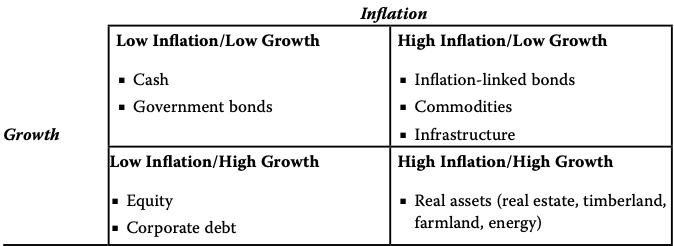
\includegraphics[scale=0.5]{/pm/macrogrowthinflation}
\caption{Growth and inflation factor matrix for Macroecnomic factor models}
\end{figure}

\begin{definition} \hlt{Fixed-Income Fundamental Multifactor Models}\\
The fixed-income fundamental factor model has components: duration (cash to long-dated bonds), credit (government securities to high yield), currency (local, foreign developed and emerging market currencies), geography (developed and emerging markets). Components can be thought of as both macroeconomic and fundamental.\\
The below model by Dopfel ($2004$) covers three macro sectors plus high yield.
\begin{equation}
r_i = a_i + \beta_{i,1} F_{\text{Govt, Short}} + \beta_{i,2} F_{\text{Govt, Int}} + \beta_{i,3} F_{\text{Govt, Long}} + \beta_{i,4} F_{\text{Inv Grade}} + \beta_{i,5} F_{\text{High Yield}} + + \beta_{i,6} F_{\text{MBS}} + \epsilon_i \nonumber
\end{equation}
where $a_i$ is expected return, $\beta_{i,k}$ is sensitivities of factor $k$, $F_k$ is factor $k$, $\epsilon_i$ is error term.\\
Note, $\beta_{i,k}$ is estimated by constrained regression (weights add up to $100\%$) of portfolio returns against factors. The factor sensitivities $\beta_{i,k}$ are standardised attributes, which is similar to computation of $z$-statistics from standard normal distribution (i.e., $\text{Sensitivity} = \frac{\text{Value} - \text{Average of Cross Section or Group}}{\text{Standard Deviation of Cross Section or Group}}$).
\end{definition}

\begin{figure}[H]
\centering
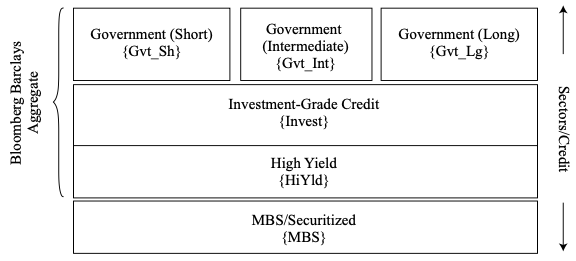
\includegraphics[scale=0.5]{/pm/fiframework}
\caption{Fixed-Income fundamental framework}
\end{figure}

\begin{remark} \hlt{Macroeconomic Factor Model versus Fundamental Factor Model}
\begin{enumerate}[label=\roman*.]
\setlength{\itemsep}{0pt}
\item Sensitivities $\beta$: in fundamental factor model, standardised sensitivites are computed directly from attribute data. In macroeconomic factor model, sensitivities are regression slope estimates.
\item Interpretation of Factors $F$: in macroeconomic factor model, the factors are surprises. In fundamental factor model, the factors are rates of return associated with each factor, estimated with multiple regression.
\item Intercept Term: in macroeconomic model, this is the expected return from an equilibrium pricing model such as APT. In fundamental factor model, the intercept has no economic interpretation; it is the regression intercept necessary to make the unsystematic risk of asset equal to zero.
\end{enumerate}
\end{remark}

\begin{definition} \hlt{Risk and Style Multifactor Models}\\
Approach incorporates risk and style factors, which can be applied across asset classes.\\
\begin{tabularx}{\textwidth}{p{4em}|p{8em}|X|X|X|X|X}
\hline
\rowcolor{gray!30}
& Factor & Equity & Credit & Treasury & Commodities & Currency \\
\hline
Macro & Economic Growth & \checkmark \checkmark &  \checkmark & & & \\
& Rates & & \checkmark & \checkmark \checkmark & & \\
& Inflation & & & \checkmark & \checkmark \checkmark & \checkmark \\
\hline
Style & Value & \checkmark \checkmark & \checkmark & & \checkmark & \checkmark \\
& Size & \checkmark \checkmark & & & &\\
& Momentum & \checkmark \checkmark & \checkmark \checkmark & \checkmark \checkmark & \checkmark \checkmark & \checkmark \checkmark \\
& Carry & \checkmark & \checkmark \checkmark & \checkmark \checkmark & \checkmark \checkmark & \checkmark \checkmark \\
& Low-Volume & \checkmark \checkmark & \checkmark & & & \\
\hline
\end{tabularx}
Double check marks denote strong alignment between risk factor and asset.\\
Single check mark denote moderate alignment.
\end{definition}

\begin{remark} \hlt{Return Attribution with Multifactor Models}\\
Can be used to attribute active manager's return to different factors.\\
Active return is difference in return between managed portfolio and benchmark.
\begin{equation}
r_{\text{Active}} = r_{\text{Portfolio}} - r_{\text{Benchmark}} \nonumber
\end{equation}
Active return may be decomposed into factor return (factor exposures differing from benchmark) and security selection (different weight chosen for specific securities compared to benchmark).
\begin{align}
r_{\text{Active}} &= r_{\text{Factor}} + r_{\text{Security Selection}} \nonumber \\
r_{\text{Factor}} &= \sum\limits_{i=1}^{K} (\beta_{i, \text{Portfolio}} - \beta_{i, \text{Benchmark}}) \times r_{i, \text{Factor}} \nonumber
\end{align}
Note that the security selection return is the residual difference between active return and factor return.
\end{remark}

\begin{remark} \hlt{Risk Attribution with Multifactor Models}\\
Active risk is the standard deviation of active return.
\begin{equation}
\sigma_{\text{Active}} = \text{Tracking Error} = \sigma(r_{\text{Portfolio}} - r_{\text{Benchmark}}) \nonumber
\end{equation}
Active risk may be decomposed into
\begin{enumerate}[label=\roman*.]
\setlength{\itemsep}{0pt}
\item Active Factor Risk: risk from active factor tilts attributable to deviations of portfolio factor sensitivities from benchmark factor sensitivities.
\item Active Specific Risk: risk from active asset selection attributable to deviations of portfolio individual asset weightings versus benchmark individual asset weightings.
\end{enumerate}
\begin{align}
\sigma_{\text{Active}}^2 &= \sigma_{\text{Factor}}^2 + \sigma_{\text{Specific}}^2 \nonumber \\
\sigma_{\text{Specific}}^2 &= \sum\limits_{i=1}^n (w_{i, \text{Portfolio}} - w_{i, \text{Benchmark}})^2 \sigma^2_{\epsilon i} \nonumber
\end{align}
where $w_{i, \text{Portfolio}}, w_{i, \text{Benchmark}}$ is weights of $i$th security in active and benchmark, $\sigma^2_{\epsilon i}$ is residual risk of $i$th asset.\\
Active factor risk is residual difference between active risk and factor risk.
\end{remark}

\begin{remark} \hlt{Applications of Multifactor Models}
\begin{enumerate}[label=\roman*.]
\setlength{\itemsep}{0pt}
\item Passive Management: tracking portfolio may be used to track an index, with a set of factor exposures constructed to match a predetermined benchmark
\item Active Management: factor portfolio may be constructed to have sensitivity $=1$ for only one risk factor, and sensitivity $=0$ for remaining factors. These are useful for speculation or hedging.
\item Rules-Based Active Management: strategies use rules to mechanically tilt factor exposures when constructing portfolios, hence introducing bias in the portfolio relative to value-weighted benchmark indices.
\end{enumerate}
\end{remark}

\begin{definition} \hlt{Carhart Four-Factor Model}\\
Extends Fama-French Three-Factor Model to include momentum
\begin{equation}
E[r_{\text{Portfolio}}] = r_{\text{Risk Free}} + \beta_{1, \text{Portfolio}} \text{RMRF} + \beta_{2, \text{Portfolio}} \text{SMB} + \beta_{3, \text{Portfolio}} \text{HML} + \beta_{4, \text{Portfolio}} \text{WML} \nonumber
\end{equation}
where $\beta$ is sensitivity of the portfolio to the factor,\\
RMRF $=$ returns on value-weighted equity index in excess of one-month T-bill rate,\\
SMB $=$ returns on small market cap minus returns on big market cap,\\
HML $=$ returns on high book-to-market stocks minus returns on low book-to-market stocks,\\
WML $=$ returns on winners minus returns on losers, a momentum factor.
\end{definition}

\begin{remark} \hlt{Benefits of Consideration in Multiple Risk Dimensions}\\
Investors choose a combination of risk-free asset and market portfolio depending on risk tolerance. Multifactor models allow investors to zero in on risks that investor has comparative advantage in bearing, and avoid risks that investor is incapable of absorbing. The models also help investors select more efficient portfolios.
\end{remark}

\begin{definition} \hlt{Information Ratio (IR)}\\
Analogous to Sharpe measure that evaluates absolute returns. Information ratio (IR) evaluates mean active returns per unit of tracking risk. The historical (ex post) IR is then
\begin{equation}
\text{IR} = \frac{\overline{r}_{\text{Portfolio}} - \overline{r}_{\text{Benchmark}}}{\sigma(r_{\text{Portfolio}} - r_{\text{Benchmark}})} \nonumber
\end{equation}
\end{definition}